\documentclass[twoside,11pt]{report}
\usepackage[utf8]{inputenc}
\usepackage{graphicx}
\usepackage[a4paper,width=150mm,top=25mm,bottom=25mm,bindingoffset=6mm]{geometry}
\usepackage{gensymb}
\usepackage{multirow}
\usepackage{amsmath}
\usepackage{pgf}
\usepackage[english,spanish,activeacute,]{babel}
\usepackage[some]{background}
\usepackage[hyphens, spaces,obeyspaces]{url}
\usepackage[breaklinks]{hyperref}
\usepackage{subfig}
\usepackage{adjustbox}
\usepackage{fancyhdr}
\usepackage[style=ieee,block=ragged]{biblatex}
\usepackage{csquotes}
\usepackage{float}
\usepackage[version=4]{mhchem}
\usepackage{chemfig}
\usepackage{silence}
\usepackage{subfiles}
\usepackage[justification=centering]{caption}
\WarningsOff[gensymb]
\addbibresource{{Documento_Latex/Referencias/references.bib}}
\graphicspath{{Documento_Latex/Imagenes/}} 



\raggedbottom


\backgroundsetup{scale=1,color=black,opacity=0.05,angle=0,contents={%
  
\includegraphics[width=0.5\paperwidth]{Documento_Latex/Imagenes/logo.png}}%
 }

\makeatletter
\newcounter{reaction}
%%% >> for report and book >>
\renewcommand\thereaction{R\,\thechapter.\arabic{reaction}}
\@addtoreset{reaction}{chapter}
\newcommand\reactiontag{\refstepcounter{reaction}\tag{\thereaction}}
\newcommand\reaction@[2][]{\begin{equation}\ce{#2}%
\ifx\@empty#1\@empty\else\label{#1}\fi%
\reactiontag\end{equation}}
\newcommand\reaction@nonumber[1]{\begin{equation*}\ce{#1}%
\end{equation*}}
\newcommand\reaction{\@ifstar{\reaction@nonumber}{\reaction@}}
\makeatother

\DeclareUnicodeCharacter{2212}{-}
\linespread{1.5}

\fancyfoot{}
\fancyfoot[LE,RO]{\thepage}
\fancyhead[RE,LO]{CHAPTER \thechapter.}


\title{Development of a Computational Desing Tool for Polypropylene-based composites having oxygen scavengers using the Hetereogenous Film Approach}
\author{Daniel Rozo}
\date{\Today}

\begin{document}



\section{Numerical Resolution Methodology}\label{subsec:numerical_methodology.}
To obtain a solution to the models presented in  the previous section, given the complexity of the system of differential equations to be solved, there exists the necessity of using numerical methods. Even though these methods do not enable us to find the exact solution of the problem, it does enables us to obtain an approximation of the analytical solution within an error interval, which depends on the implementation of the solution algorithm. In this case, given that the system of partial differential equations (PDE) which is needed to be solved is one dimensional, this system is going to be solved using finite differences techniques. These methods are based on the approximation of the definition of derivative to a finite difference, which can be solved algebraically (Equation \ref{eq:fin_dif}).

\begin{equation}
    \frac{df}{dx}\approx \frac{f(x_{i+1})-f(x_{i}) }{\Delta x}
    \label{eq:fin_dif}
\end{equation}

To use this technique, the domains in which the equations are going to be solved must be discretized. With this in mind, the spacial domain $x$ in which the diffusion and reaction of oxygen take place becomes $x_i$, which are $n$ discrete points that represent the whole domain. In the same way, time $t$ becomes $t_j$ where $0<j<m$, being $m$ the total number of steps taken in the time interval which is going to be solved. For solving the system of equations which describe the film oxygen scavenging dynamics different finite-difference algorithms were evaluated to find which of these methods was able to solve the diffusion-reaction equation in a fast and stable way. In the next subsections, the methods which were taken into account for this are going to be described, as well as how these were applied to the PDE system of the OS film. 

\subsubsection{Methods of lines}
One of the most straightforward techniques used for numerically solving PDEs is the method of lines (MOL). This method enables to transform a system of PDEs to a system of ODEs, which in turn can be solved using ODE methods such as Runge-Kutta or backward difference formula (BDF), among others. To do this all the dimensions within the PDE equation must be discretized except one. In this case, the equation which is going to be solved is
\begin{equation}
     \frac{\partial [O_2]}{\partial t}= \frac{\partial}{\partial x} \left(D_{O_2}\frac{\partial [O_2] }{\partial x}\right) -k_2[\ce{R^.}][O_2]
     \label{eq:mass_bal_dif_reacc}
\end{equation}

The variable which is going to be discretized is $x$ or the spacial dimension. This was chosen given that the only specie which has a spacial component in its mass balance is oxygen, the rest only varies along time. This implies that the reactive sites are fixed within the film. The discretization scheme chosen for the second derivative is a second-order central difference  (Equation \ref{eq:disc_diff}). 

\begin{equation}
    D_{O_2}\frac{\partial^2 [O_2]}{\partial x^2}= D_{O_2} \frac{[O_2]_{i-1}-2[O_2]_{i}+[O_2]_{i+1}}{(\Delta x)^2}
    \label{eq:disc_diff}
\end{equation}

Applying the previous equation into mass balance equation of oxygen the next expression is obtained:
\begin{equation}
     \frac{\partial [O_2]_i}{\partial t}=  D_{O_2} \frac{[O_2]_{i-1}-2[O_2]_{i}+[O_2]_{i+1}}{(\Delta x)^2} -k_2[\ce{R^.}]_i[O_2]_i.
     \label{eq:LOD_oxygen}
\end{equation}
This equation now represents an ordinary differential equation for $[O_2]_i$, which is a vector of variables of concentration of oxygen through the spacial domain which only depends on time (see Figure \ref{fig:LOD_diagram}).

\begin{figure}[ht]
    \centering
    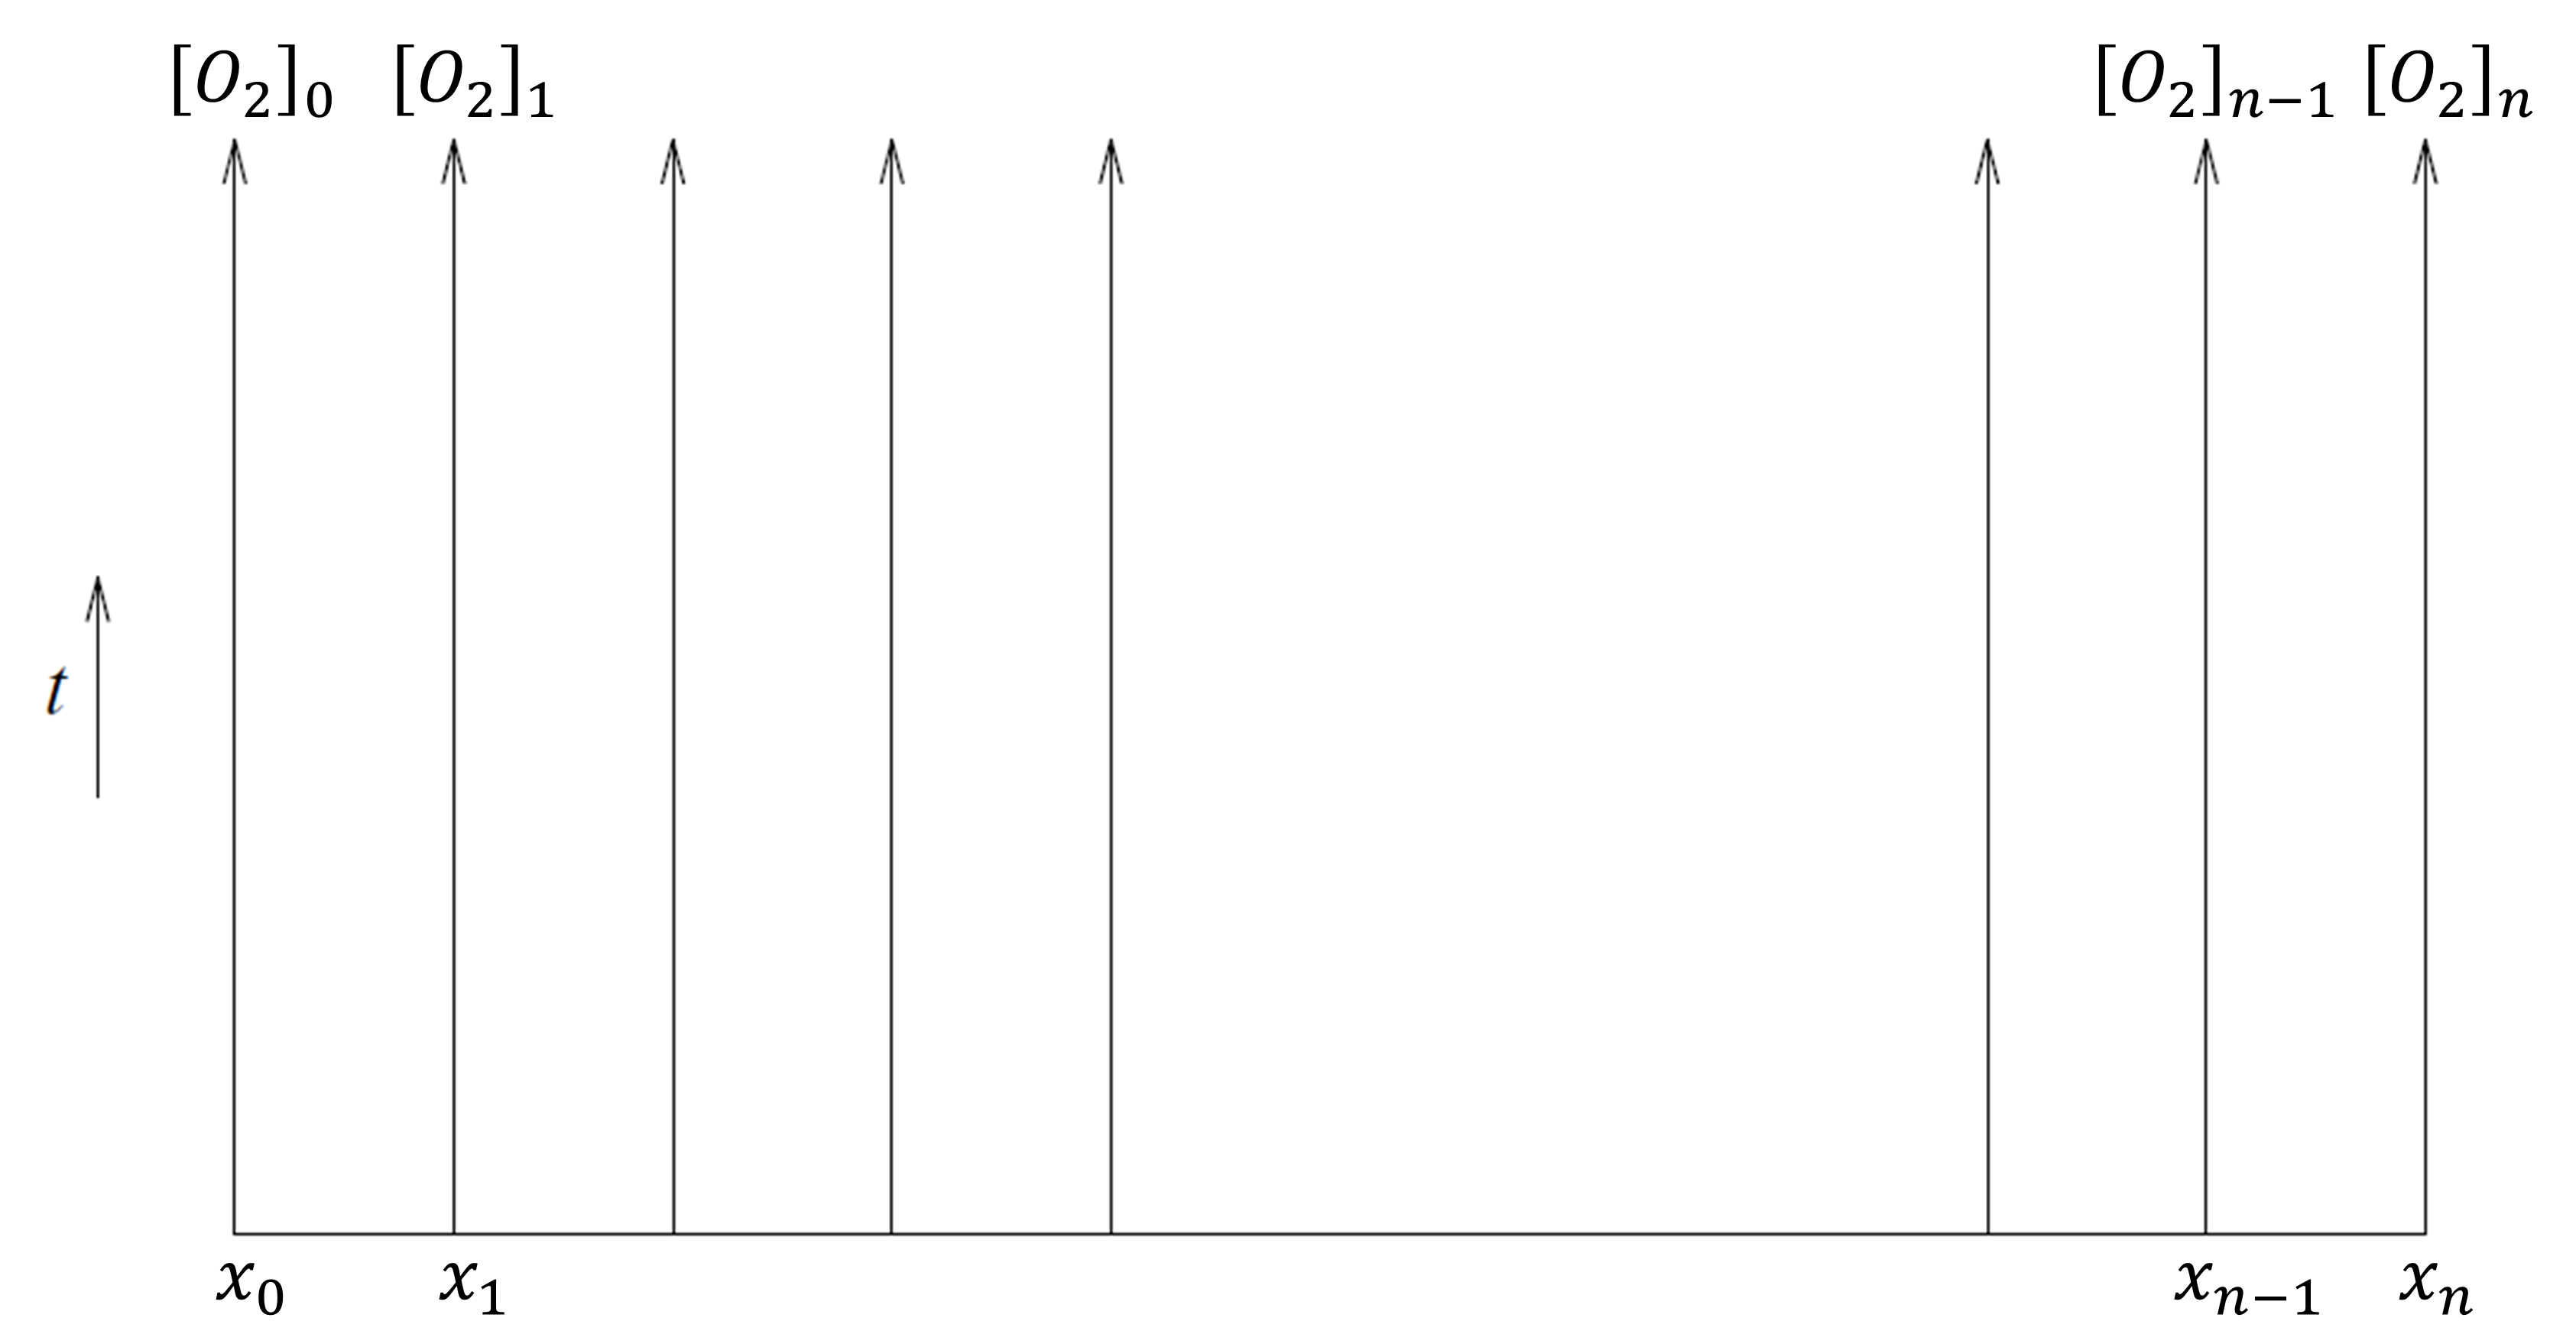
\includegraphics[width=0.7 \linewidth]{Documento_Latex/Imagenes/LOD.png}
    \caption{Method of lines interpretation. $[O_2]_i$ is the solution along the line forward in time at the grid point $x_i$. Adapted from \cite{LeVeque2007FiniteProblems}.}
    \label{fig:LOD_diagram}
\end{figure}

To solve the system of ODEs, a trapezoidal method will be used. These methods consist of calculating the time derivative at a point $t_i$ as the average of the derivative in that time step and the derivative in the next time step $t_{i+1}$. With this in mind, if the derivative of the oxygen concentration in the film with respect to time is given by equation \ref{eq:LOD_oxygen}, then in the finite difference approximation this derivative is going to be given by:

\begin{align}
    \frac{[O_2]^{j+1}_i-[O_2]^j_i}{\Delta t}=&\frac{1}{2}\Biggr(\left[ D_{O_2} \frac{[O_2]_{i-1}^{j+1}-2[O_2]_{i}^{j+1}+[O_2]_{i+1}^{j+1}}{(\Delta x)^2}-k_2[\ce{R^.}]_i^{j+1}[O_2]_i^{j+1}\right] \nonumber\\
    &-\left[D_{O_2}\frac{[O_2]_{i-1}^{j}-2[O_2]_{i}^{j}+[O_2]_{i+1}^{j}}{(\Delta x)^2}-k_2[\ce{R^.}]_i^{j}[O_2]_i^{j}\right]\Biggr).
\end{align}
This last equation is implicit with respect to time, given that the next time step can not be solve directly from the last step without solving a system of equations. The method implemented was implicit given that it is unconditionally stable and given the presence of the diffusive term which is stiff, an implicit method is required so that the method can be solve using greater time step.  The method of trapezoid when applied to LOD with a second derivative, coincides with the numerical method of Crank-Nicholson. To solve the previous system of equations in order to calculate a new time step, the previous function is rewritten as:

\begin{align}
    0=&\frac{[O_2]^{j+1}_i-[O_2]^j_i}{\Delta t}-\frac{1}{2}\Biggr(\left[ D_{O_2} \frac{[O_2]_{i-1}^{j+1}-2[O_2]_{i}^{j+1}+[O_2]_{i+1}^{j+1}}{(\Delta x)^2}-k_2[\ce{R^.}]_i^{j+1}[O_2]_i^{j+1}\right] \nonumber\\
    &-\left[D_{O_2}\frac{[O_2]_{i-1}^{j}-2[O_2]_{i}^{j}+[O_2]_{i+1}^{j}}{(\Delta x)^2}-k_2[\ce{R^.}]_i^{j}[O_2]_i^{j}\right]\Biggr),
\end{align}
which is equivalent to 
\begin{equation}
    0=F([O_2]^{i+1}). 
\end{equation}
So to find the root for the last equation will mean to calculate the next time step. This was done using the function \textit{fsolve} of the \textit{scipy} library of python 3.8, using as initialization the vector of concentration of the previous time step $[O_2]^{i}$. The initialization was chosen so that the solver converges quickly into a solution given that the profile will not change drastically in one time step. This was done for each time step until the final time $t_m$ was reached. It is important to highlight that both time and space have a uniform discretization. 

A second implementation of the LOD method was used applying the variable time step BDF method. This method was evaluated given that the BDF solver method is already implemented in the \textit{scipy} library in python 3.8..To obtain more information about this implementation read reference \cite{shampine1997matlab}.

\subsubsection{Implicit-Explicit Method}
The implicit-explicit method (IMEX) is a method that has been long used for solving reaction-diffusion problems \cite{LeVeque2007FiniteProblems}. This is because generally, the reaction part of the PDE tends to be non-stiff, which is why it can be solved individually by an explicit method, which is simpler to implement and does less work per time step than an implicit scheme. Given that the diffusion part of the equation is stiff, the use of an explicit method to solve the whole PDE is not viable, because it would require excessively small time steps for the method to be stable. In that sense, it is possible to think that an explicit treatment can be given to the reaction part of the PDE, while providing an implicit treatment to the diffusive component of it. In this way, less computational time and effort will be needed to solve the whole PDE given. This is the principle under which IMEX schemes are created. There exist several methods that apply the IMEX schemes; this depends on the treatment given to the implicit and explicit part. In this project, four IMEX schemes were evaluated.

The first and most simple IMEX method evaluated was the first order semi-implicit backward differentiation formula (1-SBDF). This scheme is based on the application of the BDF method to solve the diffusive part of the reaction implicitly while using a simple forward Euler method for the reactive part. Applying this algorithm to the oxygen mass balance equation \ref{eq:mass_bal_dif_reacc} the next expression is obtained \footnote{for the sake of simplicity, the operator of second-order centered difference will be defined for the rest of the document as $\nabla^2 [O_2]^j_i=\frac{[O_2]_{i-1}^{j}-2[O_2]_{i}^{j}+[O_2]_{i+1}^{j}}{(\Delta x)^2}$}:

\begin{equation}
   \frac{[O_2]^{j+1}_i-[O_2]^j_i}{\Delta t}=-k_2[\ce{R^.}]_i^{j}[O_2]_i^{j}+ D_{O_{2_i}}\nabla^2[O_2]_i^{j+1}.
\end{equation}
This method has the advantage of using less memory than the second-order schemes and it is more stable against high-frequency spatial errors \cite{Ruuth1995Implicit-explicitFormation}. The next three IMEX algorithms considered were the Crank-Nicholson Adam-Bashford method (CNAB, equation \ref{eq:CNAB}), the modified CNAB (MCNAB, equation \ref{eq:MCNAB}) and a second-order SBDF method (2-SBDF, equation \ref{eq:2-SBDF}). The first method, CNAB, has a small truncation error but, at the same time, does not have a good response to high-frequency error components.
    \begin{align}
    \frac{[O_2]^{j+1}_i-[O_2]^j_i}{\Delta t}=& \frac{1}{2}\Biggr[-k_2(3[\ce{R^.}]_i^{j}[O_2]_i^{j}-2[\ce{R^.}]_i^{j-1}[O_2]_i^{j-1})+\nonumber\\ &D_{O_{2_i}}(\nabla^2[O_2]_i^{j+1}+\nabla^2[O_2]_i^{j})\Biggr]
    \label{eq:CNAB}
    \end{align}
    
To solve the previous frequency problem there is the MCNAB, which has a better response to high-frequency errors but the price paid is that it requires additional computational work given the evaluation of $\nabla^2[O_2]_i^{j-1}$ \cite{ascher1995implicit} (Equation \ref{eq:MCNAB})
\begin{align}
  \frac{[O_2]^{j+1}_i-[O_2]^j_i}{\Delta t}=& \frac{1}{2}\Biggr[-k_2(3[\ce{R^.}]_i^{j}[O_2]_i^{j}-2[\ce{R^.}]_i^{j-1}[O_2]_i^{j-1})+\nonumber\\
  &\frac{D_{O_{2_i}}}{8}(9\nabla^2[O_2]_i^{j+1}+6\nabla^2[O_2]_i^{j})+\nabla^2[O_2]_i^{j-1})\Biggr]  
  \label{eq:MCNAB}
\end{align}
The last method evaluated, 2-SBDF has a larger truncation error than the CNAB, and MCNAB but it is the most stable of both methods and it does not require to evaluate any operator over $[O_2]_i^{j-1}$ (Equation \ref{eq:2-SBDF}).

\begin{align}
    \frac{3[O_2]^{j+1}_i-4[O_2]^j_i+[O_2]^{j-1}_i}{2\Delta t}=&-k_2(2[\ce{R^.}]_i^{j}[O_2]_i^{j}-[\ce{R^.}]_i^{j-1}[O_2]_i^{j-1})\nonumber\\
    &+D_{O_{2_i}}\nabla^2[O_2]_i^{j+1} 
    \label{eq:2-SBDF}
\end{align}

All second-order schemes require to know the concentration profile for the first two time steps taken, that is why for calculating the first time step the 1-SBDF method was used. 

\subsubsection{Fractional Step Methods}
In case the reactive terms of the PDE system that describes the oxygen absorption dynamics are stiff, it would require an implicit method for solving this using an acceptable time step $\Delta t$. Given that the diffusion part is linear, it can be solved using a different method that the non-linear reaction term. In that way, it is convenient to split the reaction-diffusion equation into two terms, as shown in equation \ref{eq:frac_met}.

\begin{align}
        \frac{\partial [O_2]^*}{\partial t}&=D_{O_2}\frac{\partial^2[O_2]}{\partial x^2}&
        \frac{\partial [O_2]}{\partial t} &=-k_2[\ce{R^.}][O_2]^*
    \label{eq:frac_met}
\end{align}

This method is called the fractional step method (FSM), and it has the advantage that when decoupling both parts of the equation, a different solution treatment can be given for both. The case is shown in equation  \ref{eq:frac_met} is the most straightforward implementation of first-order for an FMS. The point where both terms are relate is that the result obtained for the diffusive part is used to calculate the derivative in the reactive component. In that way, for a $\Delta t$ sufficiently small, this method will approach the solution of the non-separated PDE system. For solving the fractional diffusion equation, a Crank-Nicholson algorithm was applied (Equation \ref{eq:fraction_CN}).

\begin{equation}
    \frac{[O_2]_i^*-[O_2]_i^j}{\Delta t} = \frac{1}{2}(D_{O_{2_i}}\nabla^2[O_2]_i^j + D_{O_{2_i}}\nabla^2[O_2]_i^*)
    \label{eq:fraction_CN}
\end{equation}
This equation was solved for each time-step by using the conjugate gradient algorithm (CG) implemented in the scipy library, without preconditioning and using $[O_2]_i^j$ as the initial guess value. On the other hand, concerning the method for solving the reaction fractional equation, a trapezoidal method was used.

\begin{equation}
    \frac{[O_2]_i^{j+1}-[O_2]_i^*}{\Delta t}= -k_2 \frac{1}{2}([\ce{R^.}]_i^j[O_2]^*-[\ce{R^.}]_i^{j+1}[O_2]^{j+1}) \label{eq:fraction_trapz}
\end{equation}

As in the case of the LOD method, equation \ref{eq:fraction_trapz} was solve by rewriting the equation to the form $F([O_2]^{j+1})=0$ and finding the root of the equation with the function \textit{fsolve} of \textit{scipy}. 

\subsubsection{Adaptive Time-step Algorithm}
A disadvantage of implementing the previous numerical methods with a constant time step is that they would take a longer computational time because they will always do the same amount of iterations no matter what the final time is. In this case, given that the objective of solving the PDE system of equations for the OS film is to predict the results of the head-space test, the time-lapse over which the solution is going to be needed is of the order of 100h. In that sense, having time steps of the order of 1 second would reduce numerical error but it implies a great amount of computational time to get to the final result. As a solution to the problem of long computational times, the implementation of a variable time step algorithm is proposed. This implementation was taken from the algorithm developed by Janneli and Fazio \cite{Jannelli2006AdaptiveComplexity}, which consist of defining a criteria variable $\eta^j$ as
\begin{equation}
    \eta^j= \frac{||u^{j+1}-u^{j}||}{||u^{j}||+\varepsilon_M}.
\end{equation}
Where $u^j,u^{j+1} $ would be the whole concentration vector at the time $t^j$ and $t^{j+1}$ respectively, and $\varepsilon_M$ is a parameter which is of the order of the rounding unit so that in case that $||u^{j}||=0$ the monitor function $\eta^j$ is still well defined. This function can be interpreted as the relative change of the solution in the next time step with respect to the solution in the actual time. For numerical stability  it is desired that the value of $\eta^j$ is between a certain range $ \eta_{min}<\eta^j <\eta_{max}$. The basic guidelines so that this occurs is that for a given time step $\Delta t^j$ if the quantity is between $ \eta_{min}<\eta^j <\eta_{max}$ the new solution is accepted and the next time step $\Delta t^{j+1}$ remains equal to the actual one. In the case where $\eta^j<\eta_{min}$ then the new solution $u^{j+1}$ is accepted and the new time step is increased by a factor of $\rho$. But in the case $ \eta_{max}<\eta^j$, the solution $u^{j+1}$ calculated is not accepted and a new solution must be calculated with a reduced time step $\sigma \Delta t^j$, being $\sigma$ the factor by which the actual time step is reduced. This verification is made for every time step until the getting to the final time $t_m$. This algorithm was implemented for the LOD and FMS method described in the previous section with the parameter shown in Table \ref{tab:parameters_vari_time _Step}.


\begin{table}[H]
\centering
\caption{Variable step algorithm parameters used for the implementation of  the LOD and FSM methods. This values were determined by observation.}
\label{tab:parameters_vari_time _Step}
\begin{tabular}{|c|c|c|}
\hline
Parameters             & LOD          & FSM         \\ \hline
$\eta_{min}$           & $8x10^{-10}$ & $1x10^{-8}$ \\ \hline
$\eta_{max}$           & $1x10^{-4}$  & $1x10^{-4}$ \\ \hline
$\varepsilon_M$        & 0            & 0           \\ \hline
$\sigma$               & 0.66         & 0.2         \\ \hline
$\rho$                 & 1.5          & 2           \\ \hline
$\Delta   t_{min}$ (s) & 0.001        & 0.001       \\ \hline
$\Delta   t_{max}$ (s) & 500          & 1000        \\ \hline
$\Delta t_o$   (s)     & 0.001        & 0.001       \\ \hline
\end{tabular}%
\end{table}

\printbibliography

\end{document}